\documentclass[12pt,a4paper]{article}
\usepackage{datetime} 
\usepackage[T1]{fontenc}
\usepackage[utf8]{inputenc}
\usepackage{graphicx} 
\usepackage{url}
\graphicspath{{images/}} 
\usepackage{hyperref}
\renewcommand{\figurename}
\newline
\title{\bf\fontsize{12pt}{14pt}\selectfont KÜTAHYA SAĞLIK BİLİMLERİ ÜNİVERSİTESİ \\ MÜHENDİSLİK VE DOĞA BİLİMLERİ FAKÜLTESİ}
\date{}
\begin{document}
	
	\maketitle

	\begin{center}
			
\includegraphics{ksbu.png}
	\end{center}

	
	\begin{center}
		\vspace{1cm} 
	\end{center}
	\begin{center}
	\title{\bf\fontsize{12pt}{14pt}\selectfont YAPAY ZEKA DERSİ }
	\end{center}
		\begin{center}
		\title{\bf\fontsize{12pt}{14pt}\selectfont OPTİMİZASYON ALGORİTMALARINDAN YAPAY ARI KOLONİSİ İNCELENMESİ}
	\end{center}
	\begin{center}
	\vspace{1cm} 
	\end{center}
	\begin{center}
		
	\author{\bf\fontsize{12pt}{14pt}HASAN GÖÇER\hspace{1.5cm}2118121021}
	
	\begin{center}
	\vspace{1cm} 
	\end{center}
	\date{\today} 
	\end{center}
  
	\begin{enumerate}
	\item{\bf\fontsize{12pt}{14pt}\selectfont
 Giriş/Amaç}\newline\newline
Son yıllarda teknolojik gelişmeler, büyük miktarda verinin veritabanlarında saklanmasını sağlamıştır. Bu verilerin etkin ve doğru bir şekilde analizi, çeşitli uygulama alanlarında karar verme süreçlerine önemli katkılar sağlayabilir. Ancak, manuel çabalar genellikle yetersiz kalır. Bu nedenle, veri analizinde başarı ve anlamlı örüntülerin çıkarılması için otomatik veya yarı-otomatik teknikler geliştirilmesi gerekmektedir.

Son yıllarda, araştırmacılar sosyal böceklerin davranışlarını inceleyerek sürü zekası kavramını kullanarak yapay sistemler geliştirmeye başlamışlardır. Bu çerçevede, arı koloni optimizasyonu gibi algoritmalar ön plana çıkmıştır. Yapılan çalışmalar, arı koloni optimizasyonunun diğer sürü zekası algoritmalarına göre daha doğru sonuçlar verdiğini göstermektedir.

Bu proje, veri madenciliği problemlerini çözmek için yeni yapay arı algoritması (ABC - Artificial Bee Colony) tabanlı veri madenciliği algoritmalarının geliştirilmesini amaçlamaktadır. Bu kapsamda, ABC algoritmasının analizi yapılmış ve darboğazları belirlenmiştir. Daha sonra paralel ABC algoritması geliştirilerek hızlandırılması amaçlanmıştır. Ayrıca, ABC-tabanlı sınıflandırma algoritması ve işbirlikçi ABC-tabanlı sınıflandırma algoritması geliştirilerek çeşitli veri madenciliği sınıflandırma problemlerine uygulanmıştır.

Elde edilen sonuçlar, uluslararası konferans ve dergilerde sunulmuş ve yayınlanmıştır. Bu çalışmalar, yapay arı algoritması temelli veri madenciliği algoritmalarının etkinliğini ve performansını değerlendirmektedir.
\newline\newline\newline
 \item{\bf\fontsize{12pt}{14pt}\selectfont Literatür Araştırması} \newline
	
Literatürde arı algoritmalarının teorisi ve uygulama alanları geniş bir çerçevede incelenmiştir. Bu algoritmalar, çeşitli problemlerin çözümünde kullanılmıştır ancak özellikle çok boyutlu problemlerin çözümünde bazı sınırlılıklar ortaya çıkmıştır. Örneğin, Virtual Bee algoritması iki boyutlu nümerik problemler için geliştirilmiş olsa da çok boyutlu problemlerde yetersiz kalmıştır. Benzer şekilde, Yapay Arı Kolonisi ve diğer arı algoritmaları da ölçeklenebilirlik sorunları yaşamış ve büyük veritabanlarında düşük performans sergilemiştir.

Farklı araştırmacılar tarafından geliştirilen arı algoritmaları çeşitli alanlarda kullanılmıştır. Örneğin, yapay arı koloni algoritması yapay sinir ağlarının eğitimi için önerilmiş, ancak literatürdeki diğer populasyon-tabanlı yaklaşımlarla karşılaştırıldığında bazı sınırlılıkları olduğu görülmüştür. Benzer şekilde, arı algoritmaları robot kontrolü, protein oluşumlarının tahmini ve gezgin satıcı problemlerinin çözümü gibi farklı uygulamalarda da kullanılmıştır.

Ayrıca, veri madenciliği alanında arı algoritmalarının kullanımı da incelenmiştir. Genetik algoritma, karınca kolonisi algoritması ve parçacık sürü optimizasyonu gibi çeşitli sezgisel algoritmalar kullanılarak sınıflandırma algoritmaları geliştirilmiştir. Bunların yanı sıra, işbirlikçi yaklaşımlar da literatürde çalışılmış ve bazı algoritmalar önerilmiştir.

Ancak, geliştirilen arı algoritmalarının büyük ve çok değişkenli veri kümelerini analiz etmede ve gerektiğinde hızlı çözümler üretmede yetersiz kaldığı görülmüştür. Bu nedenle, bu algoritmaların veri madenciliği problemlerine uygulanması sınırlı kalmıştır.

Bu bağlamda, bu çalışmada paralel ABC algoritması ve iki adet ABC sınıflandırması önerilmiştir. Bu önerilen yöntemler, arı algoritmalarının performansını artırmayı ve daha geniş bir problem yelpazesine uygulanabilirliğini sağlamayı amaçlamaktadır. \cite{marine taffou}
\vspace{\baselineskip}
\vspace{\baselineskip}
\vspace{\baselineskip}
 \item {\bf\fontsize{12pt}{14pt}\selectfont METODOLOJİ }\newline \newline
{\bf\fontsize{10pt}{12pt}\selectfont İlk İzleme (Initialization):}
Başlangıçta, problem için rastgele bir çözüm kümesi (arı popülasyonu) oluşturulur. Bu çözümler genellikle rasgele seçilir veya belirli bir strateji kullanılarak oluşturulur.\newline
{\bf\fontsize{10pt}{12pt}\selectfont Bal Üretimi (Employed Bees Phase):}
Bu aşamada, her arı mevcut çözümleri gözden geçirir ve yeni çözümler üretmek için bir takım heuristikler kullanır. Bu yeni çözümler "komsu çözümler" olarak adlandırılır.
Komsu çözümler, mevcut çözümlerin değiştirilmiş versiyonlarıdır. Örneğin, bir çözümdeki bir parametre değeri değiştirilerek yeni bir çözüm elde edilebilir.\newline \newline \newline
{\bf\fontsize{10pt}{12pt}\selectfont Bal Komsu Çözüm Seçimi (Onlooker Bees Phase):}
Bu aşamada, diğer arılar (gözcü arılar) mevcut çözümleri gözden geçirir ve bu çözümler arasından en iyi olanları seçerler.
Seçim sürecinde, çözümlerin uygunluk değerleri dikkate alınır. Daha yüksek uygunluk değerlerine sahip çözümler, daha fazla tercih edilir.\newline
{\bf\fontsize{10pt}{12pt}\selectfont Yerel Arama (Local Search):}
Seçilen çözümler üzerinde yerel arama yapılabilir. Bu, daha iyi bir çözüm bulmak için mevcut çözümleri biraz daha iyileştirmeyi içerir.\newline
{\bf\fontsize{10pt}{12pt}\selectfont Grev (Scout Bees Phase):}
Bir arı, belirli bir süre boyunca daha iyi bir çözüm bulamazsa, "grev" yapar ve rastgele yeni bir çözüm üretir.
Bu, çözümün bir tür yerel minimuma sıkışmış olabileceği durumlarda çözümlerin çeşitliliğini artırmak için yapılır. \newline
{\bf\fontsize{10pt}{12pt}\selectfont Yineleme (Iteration):}
Yukarıdaki adımlar belirli bir iterasyon sayısı veya belirli bir durma kriteri sağlanana kadar tekrarlanır.
Her iterasyonda, daha iyi çözümler bulunmaya çalışılır ve popülasyonun iyileşmesi sağlanır.\newline
{\bf\fontsize{10pt}{12pt}\selectfont Sonuç (Result):}
Algoritma sonuçlandığında, en iyi bulunan çözüm veya çözümler elde edilir.
\newline
  \begin{figure}[h]
  	\caption{GANTT CHART}
  	\vspace{1cm} 
  	\centering
  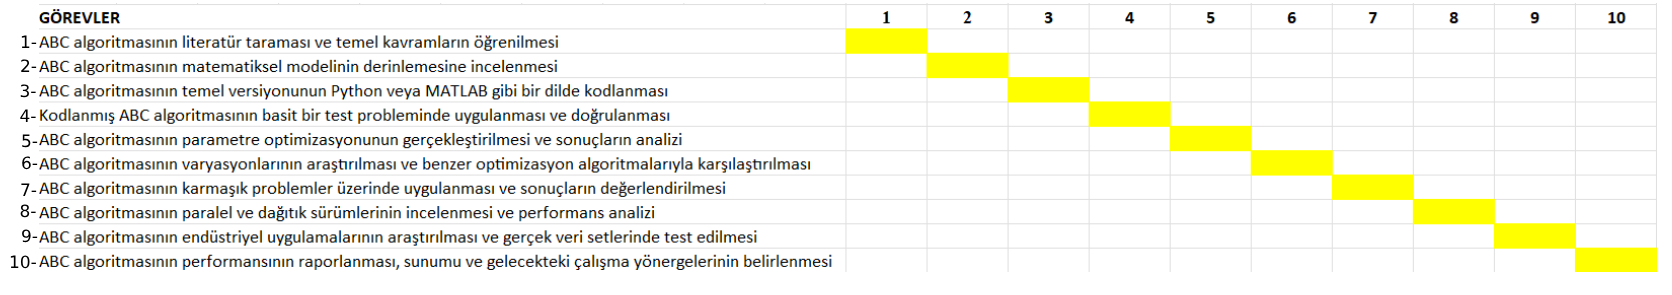
\includegraphics[width=\textwidth,height=\textheight,keepaspectratio]{gantt chart.png}
  	\label{gantt}
  		\vspace{1cm} 
  	Şekil \ref{gantt}'de görebileceğiniz üzere
  	iş akış planı gösterilmektedir.
  \end{figure}


    \end{enumerate}
\begin{itemize}

	\bibliographystyle{ieeetr}
	\bibliography{references}
  
  \bibitem{example} Modifiye Yapay Arı Koloni Algoritması ile Nümerik Fonksiyon Optimizasyonu 
  \url{ https://www.emo.org.tr/ekler/a27593adf5b4728_ek.pdf}
  
\bibitem{example} YAPAY ARI KOLONİSİ ALGORİTMASI İLE FİNANSAL
PORTFÖY OPTİMİZASYONU
  \url{http://nek.istanbul.edu.tr:4444/ekos/TEZ/53066.pdf}
  \bibitem{example}Yapay Arı Kolonisi Algoritması Kullanarak Otomatik Ders Çizelgeleme
  \url{ https://dergipark.org.tr/tr/download/article-file/193945}
 


\end{itemize} 
\end{document}
